\section{Fase di Progettazione}
    \subsection{Struttura del Sito}
    In questa sezione presentiamo una prima bozza grafica delle varie pagine del sito. Ciò ci è servito per avere un'idea generale sull'aspetto che dovrà avere il sito e per avere una base da cui partire per lo sviluppo del layout.
        
    La struttura della gerarchia del sito è suddivisa in pagine, alcune delle quali hanno delle sottopagine:
    \begin{itemize}
        \item Home;
        \item Auto a noleggio;
        \item Auto in vendita;
        \item Contatti;
        \item Pagina di Login;
        \item Pagina di Registrazione;
        \item Area privata (utente generico):
            \begin{itemize}
                \item Area personale;
                \item Dati Personali;
                \item Preventivi;
                \item Noleggi;
                \item Messaggi.
            \end{itemize}
            \item Area privata (utente amministratore):
                \begin{itemize}
                    \item Home amministratore;
                    \item Messaggi;
                    \item Veicoli a noleggio;
                    \item Veicoli in vendita;
                    \item Prenotazione veicoli.
                \end{itemize}
    \end{itemize}

    \subsection{Database}
    Viene riportata la rappresentazione del database, realizzata in fase di progettazione, durante la quale si è discussa la necessità di avere le diverse tabelle e per ogni tabella i necessari attributi, per poi utilizzarli al meglio.
    \begin{figure}[H]
        \centering
        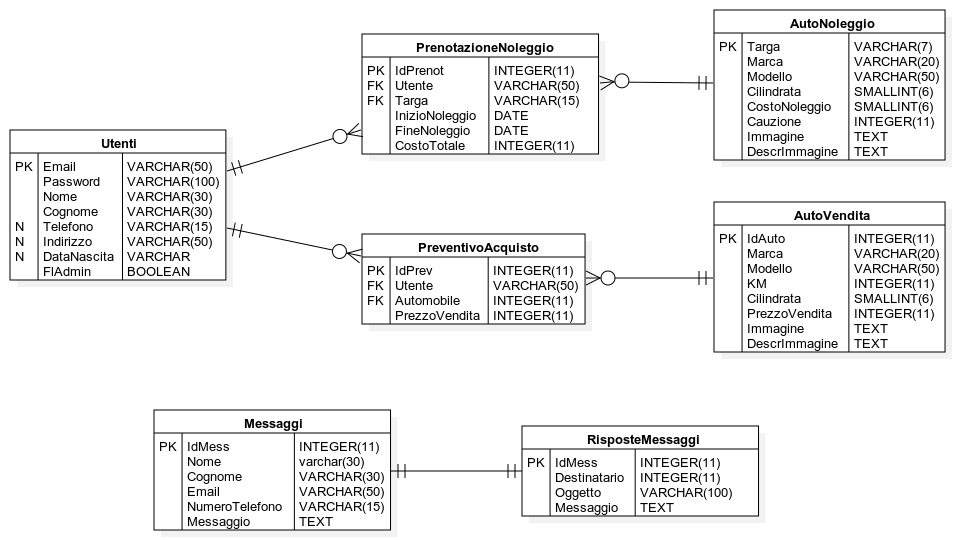
\includegraphics[width=14cm]{./img/database.png}
        \caption{Schema del database}  \label{fig:xray}
    \end{figure}
    Il database è composto dalle seguenti tabelle:
    \begin{itemize}
        \item \textbf{Utenti:} contiene i dati e le credenziali degli utenti registrati, la password è stata codificata con la funzione \textit{password\_hash} di PHP;
        \item \textbf{Messaggi:} contiene i messaggi inviati dagli utenti;
        \item \textbf{RisposteMessaggi:} contiene le risposte dell'amministratore ai messaggi inviati dagli utenti;
        \item \textbf{AutoVendita:} contiene le auto in vendita;
        \item \textbf{AutoNoleggio:} contiene le auto a noleggio;
        \item \textbf{PreventivoAcquisto:} contiene i preventivi degli acquisti delle auto effettuati dagli utenti;
        \item \textbf{PrenotazioneNoleggio:} contiene i noleggi delle auto effettuati dagli utenti;
    \end{itemize}

    \subsection{Accessibilità}
    Per garantire l'accesso al sito al maggior numero di categorie di utenti possibile sono stati adottati molti accorgimenti.
    Di seguito l'elenco dei più importanti:
    \begin{itemize}
        \item i breadcrumbs, che indicano sempre all'utente la posizione nel sito;
        \item tutti i form sono provvisti di una legenda;
        \item attributo alt nelle immagini, che rende disponibile un testo alternativo in caso in cui l’immagine non venga caricata o l'utente non sia in grado di vederla;
        \item link per saltare l'header e il menù di navigazione, nascosti di default ma visibile agli screen reader. Sono posti come primi link della pagina e consentono di navigare direttamente al contenuto della pagina. prima voce del menu, viene utilizzata nel caso in cui l’utente che utilizza lo screen reader voglia saltare direttamente al contenuto della pagina, velocizzando la navigazione;
        \item pulsante "TOP", sotto forma di bottone sempre visibile, che si trova a lato del content: se cliccato, ti porta all’inizio del content. Utile per evitare lo scroll e velocizzare la navigazione;
        \item colori ad elevato contrasto, almeno livello AA del WCAG 2.1, verificato attraverso un apposito software;
    \end{itemize}
\pagebreak